\section{Strategies}

In backward induction, a specific move must be identified at every node. 
Let $P_i$ denote the set of all nodes at which player $i$ is required to make a decision.
\begin{definition}[\textit{Pure strategy}]
    A pure strategy for player $i$ is defined as a function on the set $P_i$, which associates each node $v$ in $P_i$ with a child node $x$, or equivalently, an edge $(v, x)$.
\end{definition}
\begin{definition}[\textit{Mixed strategy}]
    A mixed strategy refers to a probability distribution over the set of pure strategies.
\end{definition}
When a player possesses $n$ pure strategies, the collection of their mixed strategies is represented as:
\[\sum_n=\left\{p=(p_1,\dots,p_n)|p_i\geq 0 \text{ and }\sum{p_i}=1\right\}\]
Here, $\sum_n$ forms the fundamental simplex in $n$-dimensional space. 

\begin{example}
    Consider the following tree: 
    \begin{figure}[H]
        \centering
        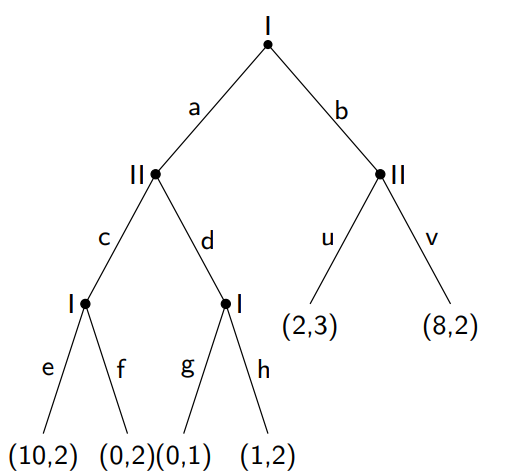
\includegraphics[width=0.75\linewidth]{images/tree2.png}
    \end{figure}
    The strategies depicted in the tree are shown below:
    \begin{figure}[H]
        \centering
        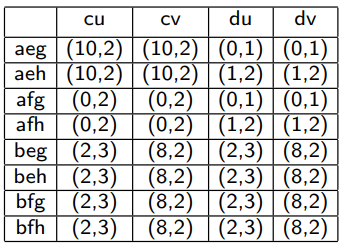
\includegraphics[width=0.75\linewidth]{images/strategies.png}
    \end{figure}
    Note that Player 1's strategies are listed in the rows, while Player 2's are in the columns. 
    All combinations are included, even if they are equivalent (e.g., strategies b-- for Player 2). 
    The table may contain repeated pairs, as different strategies can lead to the same outcomes. 
    \begin{itemize} 
        \item \textit{Extensive form}: the various moves of the players are presented sequentially. 
        \item \textit{Strategic form}: all players' strategies are presented simultaneously. 
    \end{itemize}
\end{example}

\begin{theorem}[Von Neumann on strategies]
    In the game of chess, one of the following scenarios must hold: 
\end{theorem}
\begin{enumerate}
    \item \textit{White has a winning strategy.}
    \item \textit{Black has a winning strategy.}
    \item \textit{Both players possess a strategy that guarantees at least a tie.}
\end{enumerate}
The first outcome occurs when there exists a row containing all winning elements. 
The second outcome arises when there is a column consisting of all winning elements. 
The third outcome features mixed results, including ties, but does not encompass all three outcomes in a single row or column.

If $P_i = \{v_1, \dots, v_k \}$ and $v_j$ has $n_j$ children, then the total number of strategies available to Player $i$ is $n_1 \cdot n_2 \cdot \dots \cdot n_k$. 
This illustrates that the number of strategies, even in short games, is typically quite substantial.
\begin{example}
    In the game of Tic-Tac-Toe, if the game is halted after three moves, the first player has $9 \cdot 7 ^{(8\times9)}$ strategies available (not accounting for symmetrical configurations).
\end{example}